\documentclass[11pt]{article}
\usepackage[margin=1in]{geometry}
\usepackage{amsmath,amssymb,amsthm}
\usepackage{graphicx}
\usepackage{booktabs}
\usepackage[numbers,sort&compress]{natbib}
\usepackage{xcolor}
\usepackage{enumitem}
\usepackage{url}
\usepackage[colorlinks=true,linkcolor=blue!50!black,citecolor=blue!50!black,urlcolor=blue!50!black]{hyperref}

\newtheorem{proposition}{Proposition}
\newtheorem{lemma}{Lemma}
\newtheorem{corollary}{Corollary}
\theoremstyle{definition}
\newtheorem{definition}{Definition}
\newtheorem{example}{Example}
\theoremstyle{remark}
\newtheorem{remark}{Remark}

\newcommand{\code}[1]{\texttt{#1}}

\title{When Is a Sealed-Bid Task Award Truthful?\\Composition Conditions for Procurement Auctions in On-Chain Agent Markets}
\author{Shenton Yan\\[2pt]
\small The Hong Kong Polytechnic University\\
\small \url{https://github.com/shentonyan}}
\date{October 2026}

\begin{document}
\maketitle

\begin{abstract}
Several draft Ethereum standards let autonomous agents post tasks, escrow rewards and settle on delivery, but none specifies how a task is awarded when several agents want it. We propose a sealed-bid award interface for this setting and study when its incentive properties survive composition with the escrow standard that consumes the award. Following Myerson's procurement framework, the interface separates a commit--reveal procedure from a stateless mechanism that maps revealed bids to winners and prices, and it admits four pricing rules: first-price, second-price (Vickrey), uniform-price and posted-price. Our main observation is that incentive compatibility is a property of the award together with its consumer, not of the award alone. We show that when the consumer pays a fixed reward, the only incentive-compatible rule is a posted price, and that a consumer that pays the award price must also be committed to executing every award, with the task content fixed before any bid is made. We then examine frictions specific to a public ledger. Sequential public reveals give a last revealer holding several commitments a gain of up to about 27\% of the reserve under first-price and none under second-price; requester-posted dummy commitments lower expected payment by about 19\% under first-price; and an operator bidding from two addresses can profit under uniform-price but not under single-unit second-price. The dominance results are machine-checked in Lean 4, and a Solidity reference implementation with tests accompanies a draft standard under public review.
\end{abstract}

\section{Introduction}

Markets in which software agents buy and sell work are beginning to run on public blockchains. On Ethereum, three draft standards describe the core of such a market: ERC-8183 escrows a job and releases payment on an evaluator's attestation \citep{erc8183}, ERC-8195 defines a task market with an auction mode \citep{erc8195}, and ERC-8414 turns a task into a token that holds its reward and pays whoever fulfils it \citep{erc8414}. Each standard handles posting, escrow and settlement. None of them specifies how a task is awarded when more than one agent wants it: ERC-8183 receives the outcome of an off-chain bidding process, ERC-8195 fixes the rule to lowest-bid-wins with bids relayed off-chain, and ERC-8414 leaves bidding to a companion extension. In practice each market writes its own award logic, and nobody outside can tell what an award meant or whether its price was fair.

Choosing a supplier by competitive bids is a procurement auction, and its theory is well developed. \citet{myerson1981} characterises the incentive-compatible mechanisms and the optimal one; \citet{vickrey1961} gives the second-price rule under which bidding one's true cost is a dominant strategy; revenue equivalence \citep{myerson1981,riley1981} says that the buyer's expected payment depends only on the allocation rule and the reserve. A standard can therefore fix the procedure and the allocation conditions and leave the pricing rule pluggable. What the classical theory takes for granted, however, is that the auctioneer is bound by the mechanism: the winner is paid what the mechanism says, the award is executed, and the object being sold does not change after the bids are in. In a modular on-chain market none of this is automatic. The award is computed by one contract and acted on by another, written to a different standard, with its own payment and authority rules.

This paper makes three contributions.

\begin{enumerate}[leftmargin=*,itemsep=2pt]
\item \textbf{An award interface derived from the revelation principle} (Section~\ref{sec:model}). A tender runs a commit--reveal procedure and passes the revealed bids, in commit order, to a stateless mechanism contract that returns winners and prices. We state seven conditions every mechanism must satisfy, including the monotonicity that incentive compatibility requires, and four normative pricing rules.
\item \textbf{Composition conditions} (Section~\ref{sec:composition}). We show that the incentive properties of an award rule do not transfer to the market that consumes the award unless the consumer is \emph{payment-binding} (it pays the award price) and \emph{execution-binding} (it executes every award with no discretion conditioned on revealed bids), with the task content fixed when the tender opens. If the consumer pays a fixed reward, the only incentive-compatible rule is a posted price (Proposition~\ref{prop:fixed}). These conditions lead to two declared integration profiles and to concrete adapters for ERC-8414.
\item \textbf{Frictions of a public ledger} (Section~\ref{sec:ledger}). We quantify three ways in which running the auction on a public chain departs from the sealed-bid ideal---sequential reveals, dummy commitments and multiple addresses---and show that single-unit second-price is robust to all three while first-price and uniform-price are not.
\end{enumerate}

The dominance results are proved in Lean~4 \citep{demoura2021} with no unproved assumptions, and a Solidity reference implementation is tested against the specification (Section~\ref{sec:impl}). Much of the design was shaped by public review of the draft standard \citep{thread29814}: several of the conditions in Section~\ref{sec:composition} and the false-name analysis in Section~\ref{sec:ledger} began as objections from reviewers, credited in the Acknowledgements.

\paragraph{Related work.} The mechanism-design results we rely on are standard \citep{myerson1981,riley1981,krishna2010,milgrom2004}. The importance of commitment for the auctioneer is the subject of \citet{mcafee1997}, who show how a seller who cannot commit not to re-auction loses the benefit of an optimal reserve; our execution-binding condition is the analogue for a modular system in which the party that runs the auction and the party that executes it differ. Demand reduction in multi-unit uniform-price auctions is analysed by \citet{ausubel2014}, and false-name bidding, in which one participant uses several identities, by \citet{yokoo2004}. Sealed-bid auctions on Ethereum have been implemented with cryptographic commitments and zero-knowledge proofs \citep{galal2018}; that line of work concentrates on bid privacy and verifiability, whereas we concentrate on what the award means to the contract that consumes it. Transaction ordering on public blockchains, which makes reveals observable before they are final, is documented by \citet{daian2020}.

\section{Model and Interface}
\label{sec:model}

\subsection{Procurement setting}

A requester wants a task performed and values it at $v_0$. There are $n$ bidders; bidder $i$ privately knows its cost $c_i \in [\underline{c}, \bar{c}]$, drawn independently from a distribution $F$ with density $f$. Utilities are quasi-linear: a bidder who is awarded the task and paid $p$ earns $p - c_i$, and earns zero otherwise. In procurement form the role of Myerson's virtual value is played by the \emph{virtual cost} $\psi(c) = c + F(c)/f(c)$; under the regularity condition that $\psi$ is increasing, the requester's optimal mechanism awards the task to the lowest-cost bidder if $\psi(c_{(1)}) \le v_0$, which amounts to a reserve $r = \psi^{-1}(v_0)$ \citep{myerson1981}. With costs uniform on $[0,1]$ and $v_0 = 1$, $\psi(c) = 2c$ and $r = 1/2$; we use this case for every number in the paper.

\subsection{The tender procedure}

A \emph{tender} is opened by the requester with fixed terms: a target reference naming the task in the consuming standard, the mechanism contract, the reserve $r$, the number of identical units, commit and reveal deadlines, a bond, the recipient of forfeited bonds, a cap on the number of bidders, an integration profile (Section~\ref{sec:profiles}) and a hash of the task content. Bidders then go through three phases (Figure~\ref{fig:lifecycle}).

\begin{enumerate}[leftmargin=*,itemsep=2pt]
\item \textbf{Commit.} Each bidder posts $H(\mathit{tenderId}, \mathit{bidder}, b, s)$ for its bid $b$ and a random salt $s$, and locks the bond.
\item \textbf{Reveal.} After the commit deadline, each bidder opens its commitment. The bond is returned on a valid reveal.
\item \textbf{Finalize.} After the reveal deadline, anyone may finalize. The tender passes the revealed bids, in commit order, to the mechanism, checks the result, stores the award and forfeits the bonds of bidders who never revealed.
\end{enumerate}

\begin{figure}[t]
\centering
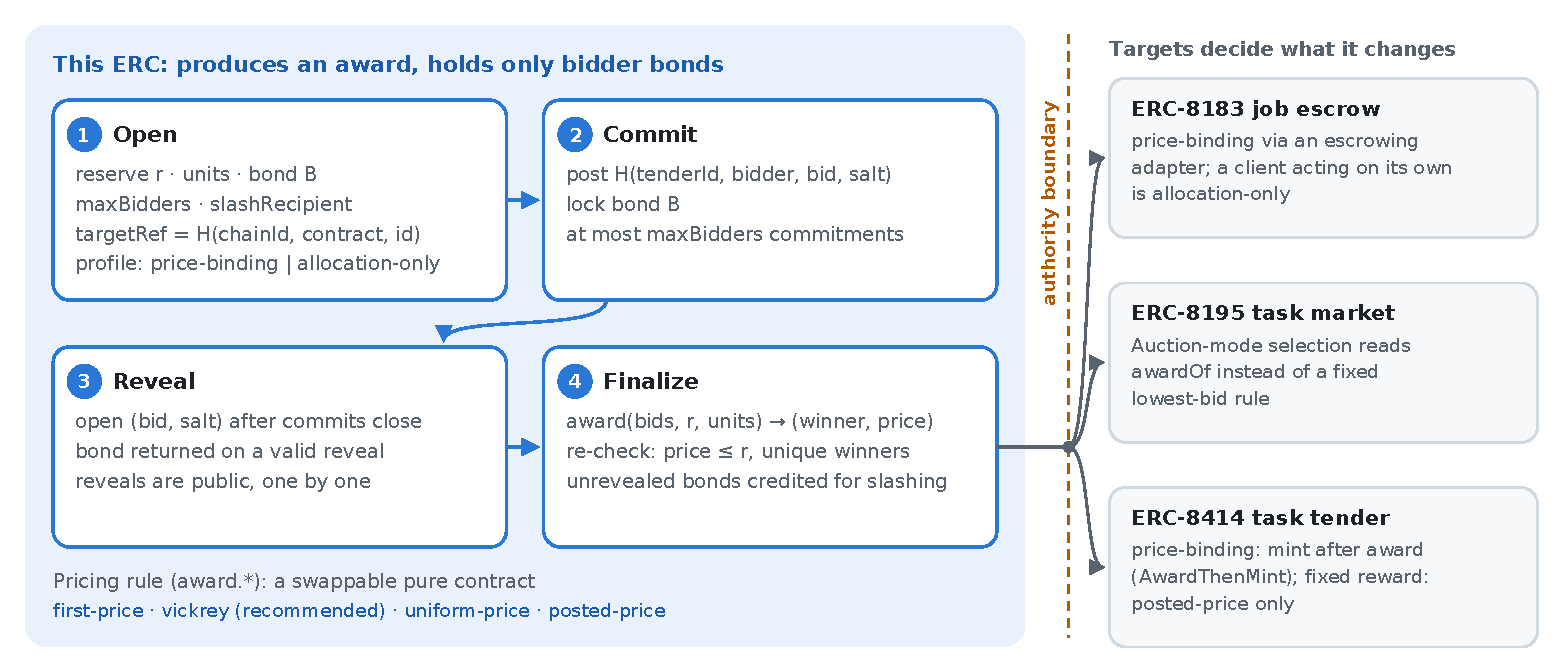
\includegraphics[width=\linewidth]{fig-lifecycle.pdf}
\caption{Lifecycle of a tender. The award crosses an authority boundary: each consuming standard decides what the award may change.}
\label{fig:lifecycle}
\end{figure}

The tender contract holds bidder bonds only. It never holds the task reward, judges a deliverable or acts on the task; whether and how an award changes the task is decided by the consuming standard. We call this the \emph{authority boundary}.

\subsection{The mechanism interface}

By the revelation principle every feasible auction is equivalent to a direct mechanism, a pair of functions from reported types to an allocation and a payment. The interface makes exactly that pair a contract: \code{award(bids, reserve, units)} returns a list of (winner, price) pairs. Each mechanism must satisfy the following conditions.

\begin{enumerate}[leftmargin=*,itemsep=1pt,label=(C\arabic*)]
\item It is deterministic and reads no state, and its output never changes over the contract's life.
\item Every winner is a bidder in the input whose bid is at most the reserve.
\item No price exceeds the reserve.
\item No winner appears twice, and there are at most \code{units} awards.
\item Lowering one bidder's bid, all else fixed, never removes that bidder from the award (monotonicity).
\item Ties on the bid go to the bid that appears earlier in the input, that is, the earlier commitment.
\item No winner is paid less than its own bid.
\end{enumerate}

Condition (C5) is the monotonicity of the allocation rule that incentive compatibility requires. Because the mechanism is a third-party contract, the tender re-checks (C2)--(C4) and (C7) against the revealed bids before storing any award; none of these checks depends on the pricing rule. The four normative rules are summarised in Table~\ref{tab:rules}.

\begin{table}[t]
\centering
\small
\begin{tabular}{@{}llll@{}}
\toprule
Rule & Winners & Price per winner & Truthful bidding \\
\midrule
first-price & lowest bid within $r$ & own bid & no \\
second-price (Vickrey) & lowest bid within $r$; one unit & $\min(r, \text{second-lowest bid})$ & dominant \\
uniform-price & $k$ lowest bids within $r$ & $\min(r, (k{+}1)\text{th lowest bid})$ & dominant per address \\
posted-price & earliest $k$ bids within $r$ & $r$ & acceptance dominant \\
\bottomrule
\end{tabular}
\caption{Normative pricing rules. For uniform-price, truthfulness assumes unit demand per bidder; Section~\ref{sec:falsename} shows what happens when one operator holds several addresses.}
\label{tab:rules}
\end{table}

Second-price is the recommended default. In the symmetric regular case, second-price with the optimal reserve is an optimal procurement mechanism, and its payment rule contains no distributional parameters, so it stays incentive compatible when the requester's beliefs about agents' costs are wrong. First-price requires each bidder to know the others' cost distribution to bid well, and agents from different operators share no common prior. The reserve is a separate term because the optimal reserve is strictly below the requester's value and the mechanism must be allowed to return no award. Table~\ref{tab:reserve} shows that its value is large in thin markets: with two bidders, the optimal reserve raises the requester's expected surplus by 25\% over a reserve equal to its value, and with ten bidders by only 0.01\%.

\begin{table}[t]
\centering
\small
\begin{tabular}{@{}rccc@{}}
\toprule
$n$ & surplus, $r = 1/2$ & surplus, $r = v_0 = 1$ & gain \\
\midrule
2 & 0.4167 & 0.3333 & 25.0\% \\
3 & 0.5312 & 0.5000 & 6.25\% \\
5 & 0.6719 & 0.6667 & 0.78\% \\
10 & 0.8183 & 0.8182 & 0.01\% \\
\bottomrule
\end{tabular}
\caption{Requester's expected surplus with the optimal reserve and with no effective reserve. Costs uniform on $[0,1]$, $v_0 = 1$. Values are exact integrals over order statistics, cross-checked by simulation.}
\label{tab:reserve}
\end{table}

\section{Composition: When the Award's Incentives Survive}
\label{sec:composition}

The incentive properties in Table~\ref{tab:rules} are properties of a mechanism, that is, of an allocation rule and a payment rule together. On-chain, the award contract computes both, but the consuming standard decides what is paid and whether anything happens at all. The payoff a bidder actually faces is that of the composition of the award with its consumer. Following a reviewer's formulation, incentive compatibility of the award does not imply incentive compatibility of the composition. This section states what the consumer must do for it to hold.

\subsection{Fixed rewards admit only a posted price}

Suppose the consumer uses the award only to choose the winner and pays a fixed reward $R$, as ERC-8414 does when a task token is minted with a fixed reward per completion. Let $Q(c)$ be a bidder's interim probability of winning when it reports cost $c$ and others report truthfully, and $X(c)$ its expected payment.

\begin{lemma}[Payment identity]
\label{lem:payment}
A direct mechanism is Bayesian incentive compatible if and only if $Q$ is non-increasing and, for some constant $K$,
\[
X(c) = c\,Q(c) + \int_c^{\bar{c}} Q(s)\,ds + K .
\]
\end{lemma}

This is the procurement form of Myerson's characterisation \citep{myerson1981}; the bidder's equilibrium utility $U(c) = X(c) - cQ(c)$ is absolutely continuous with $U'(c) = -Q(c)$.

\begin{proposition}[Fixed reward]
\label{prop:fixed}
Consider a Bayesian incentive-compatible and individually rational mechanism in which every winner is paid the same fixed amount $R$, so that $X(c) = R\,Q(c)$. Then $Q$ is constant on $[\underline{c}, R)$ and zero on $(R, \bar{c}]$. In particular, the chance of winning cannot depend on the bid below $R$: the mechanism is a posted price, with ties among acceptances broken by something other than the bid.
\end{proposition}

\begin{proof}
With $X = RQ$, the bidder's utility is $U(c) = (R - c)Q(c)$. By Lemma~\ref{lem:payment}, $U$ is absolutely continuous with $U' = -Q$ almost everywhere. On any closed interval $[a, b]$ that does not contain $R$, the function $1/(R - c)$ is smooth, so $Q = U/(R - c)$ is absolutely continuous there. Differentiating $U = (R - c)Q$ gives $U' = -Q + (R - c)Q'$ almost everywhere, and equating with $U' = -Q$ yields $(R - c)\,Q'(c) = 0$, hence $Q' = 0$ almost everywhere on $[a, b]$. An absolutely continuous function with zero derivative almost everywhere is constant, so $Q$ is constant on every such interval, and therefore on $[\underline{c}, R)$ and on $(R, \bar{c}]$. Individual rationality requires $(R - c)Q(c) \ge 0$, so $Q = 0$ on $(R, \bar{c}]$.
\end{proof}

A bid-ranking rule on top of a fixed reward does not merely fail to be truthful; it collapses. Any bidder with cost below $R$ weakly prefers the lowest admissible bid, because bidding lower never loses a win and the payment does not depend on the bid (machine-checked; see Table~\ref{tab:lean}). With every such bidder at the minimum, the tie rule awards the task to whoever committed first, which is unrelated to cost. A reviewer's example makes the failure concrete: with $R = 100$, a bidder with cost 60 facing a rival bid of 50 earns nothing by bidding 60 and earns 40 by bidding 40, which is also checked in Lean. The efficiency cost is substantial. With costs uniform on $[0,1]$ and $R = 1/2$, the expected cost of the agent that does the work is $1/4$ when the first acceptance wins, against $0.196$ under a price-binding second-price award with three bidders and $0.153$ with five: the work is done 27\% and 63\% more expensively.

The positive counterpart is that the posted price, which Proposition~\ref{prop:fixed} singles out, is incentive compatible in the strongest sense.

\begin{proposition}[Posted price]
\label{prop:posted}
Under \code{award.posted-price} with one unit, where every bid at most $r$ is an acceptance and the earliest acceptance in commit order wins at price $r$, accepting exactly when $c \le r$ is a weakly dominant strategy, for every commit position and every behaviour of the other bidders.
\end{proposition}

\begin{proof}
Whether an earlier committer accepted does not depend on the bidder's own amount. If one did, the bidder's payoff is zero whatever it bids. Otherwise it wins exactly when its bid is at most $r$ and earns $r - c$, which is non-negative exactly when $c \le r$. Machine-checked as \code{posted\_price\_acceptance\_dominant}.
\end{proof}

\subsection{Price-binding needs execution-binding}
\label{sec:profiles}

Paying the award price is necessary for the truthfulness of second-price, but it is not sufficient. If the consumer can decline an award after the reveals, it is choosing a reserve after seeing the bids, and that choice can depend on the winner's own bid.

\begin{example}
\label{ex:discretion}
A requester executes an award only if the price exceeds the winning bid by at most 10. A bidder with cost 40 faces one rival bid of 60 under second-price. Bidding 40 wins at price 60, a markup of 20, so the requester declines and the bidder earns zero. Bidding 50 wins at price 60, a markup of 10, the award is executed, and the bidder earns 20.
\end{example}

The general point is that the consumer's discretion multiplies the award's allocation by an execution indicator that depends on the bids, and the product need not be monotone in the way (C5) guarantees for the award alone. This is the modular counterpart of the commitment problem in \citet{mcafee1997}: Myerson's results assume the designer is bound by the mechanism, and without that the revealed costs also leak into whatever the requester does next. We therefore define the two conditions that a consumer must meet.

\begin{definition}
A consuming integration is \emph{payment-binding} if it pays each winner exactly its award price. It is \emph{execution-binding} if, before the commit deadline, it holds an authorisation such that, for every admissible non-empty award, the transition that executes the award at its price can be triggered by anyone, and neither the requester nor any third party can withhold it, pre-empt it or cause it to revert.
\end{definition}

The definition is stated over reachable states, not transactions: what matters is that no state is reachable in which an award is final and its execution can be withheld or made impossible. Escrowing the reserve is one way to meet the funding part of execution-binding; it does not meet the condition by itself. In building the reference adapter for ERC-8414 we found a reachable state of exactly this kind: the adapter would mint the task token at an identifier that anyone could mint first, after which settlement reverted permanently. The fix was to reserve the identifier in the adapter's own namespace when the tender opens.

A third requirement concerns what the bids price. Bidders price the task they see when they commit. If the task can change after the first commitment, before or after the award, the bids no longer price the same work, and a requester who changes it after the reveals renegotiates with the winner's revealed cost in hand. Fixing the content at award time would not suffice, since a change between the reveals and the award has the same effect. Tenders therefore commit to a hash of the task content when they open, and an award applies only to that content.

These conditions define the two integration profiles that every tender declares before anyone commits.

\begin{itemize}[leftmargin=*,itemsep=2pt]
\item \textbf{Price-binding}: the consumer is payment-binding and execution-binding and keeps the content fixed. Any pricing rule may be used, and the incentive properties in Table~\ref{tab:rules} hold.
\item \textbf{Allocation-only}: the consumer uses the winners only. By Proposition~\ref{prop:fixed}, the tender must use \code{award.posted-price}, with the reserve equal to the fixed reward.
\end{itemize}

For ERC-8414 the two profiles correspond to two adapters. An award-then-mint adapter is price-binding: the requester escrows the reserve when opening the tender; once the tender is awarded, one permissionless transition finalises it if needed, mints the task token with its reward equal to the award price, funds it from the escrow and refunds the rest; the adapter keeps the token's update authority so that the task cannot change. An award-gated verifier is allocation-only: it sits in a fixed-reward token's acceptance slot and settles a submission only if the fulfiller won a posted-price tender opened against the task's current content.

\section{Frictions of a Public Ledger}
\label{sec:ledger}

A commit--reveal procedure on a public chain is not a sealed-bid auction. Reveals are public transactions that arrive one by one, commitments are cheap to create, and the contract sees addresses rather than operators. We examine each friction in the uniform-cost case with $r = 1/2$.

\subsection{Sequential reveals}

A bidder who reveals last has seen the earlier reveals, and anyone watching a public mempool sees pending ones \citep{daian2020}. A bidder can exploit this by holding several commitments at different amounts and opening only the one that does best against what it has seen; the others forfeit their bonds. Under second-price this is worthless.

\begin{proposition}[Vickrey dominance]
\label{prop:vickrey}
Under \code{award.vickrey} with reserve $r$ and commit-order tie-breaking, for any bids of the other bidders, in any commit order, a bidder with cost $c$ earns at least as much by bidding $c$ as by any other bid, and its payoff from bidding $c$ is non-negative.
\end{proposition}

The proof is the classical one \citep{vickrey1961} adapted to the reserve and tie rule; it is machine-checked as \code{truthful\_dominant} and \code{truthful\_nonneg}. Because the truthful bid is optimal against every profile of other bids, information about those bids has no value, and every extra commitment strictly loses its bond.

Under first-price the information is valuable. We model a deviant that holds $k$ commitments evenly spaced between its equilibrium bid and the reserve, reveals last, and opens the highest commitment below the lowest rival bid it has seen, while rivals bid as in a sealed first-price auction. Figure~\ref{fig:ladder} and Table~\ref{tab:ladder} show the gain. With three to five bidders it approaches 27\% of the reserve. Deterring even a two-commitment ladder requires a bond of 10 to 12.5\% of the reserve when there are three or fewer bidders. Because a better-placed ladder gains more, these bond figures are lower bounds. Deployments that use first-price should make reveals simultaneous, for instance through threshold encryption, rather than rely on the bond.

\begin{figure}[t]
\centering
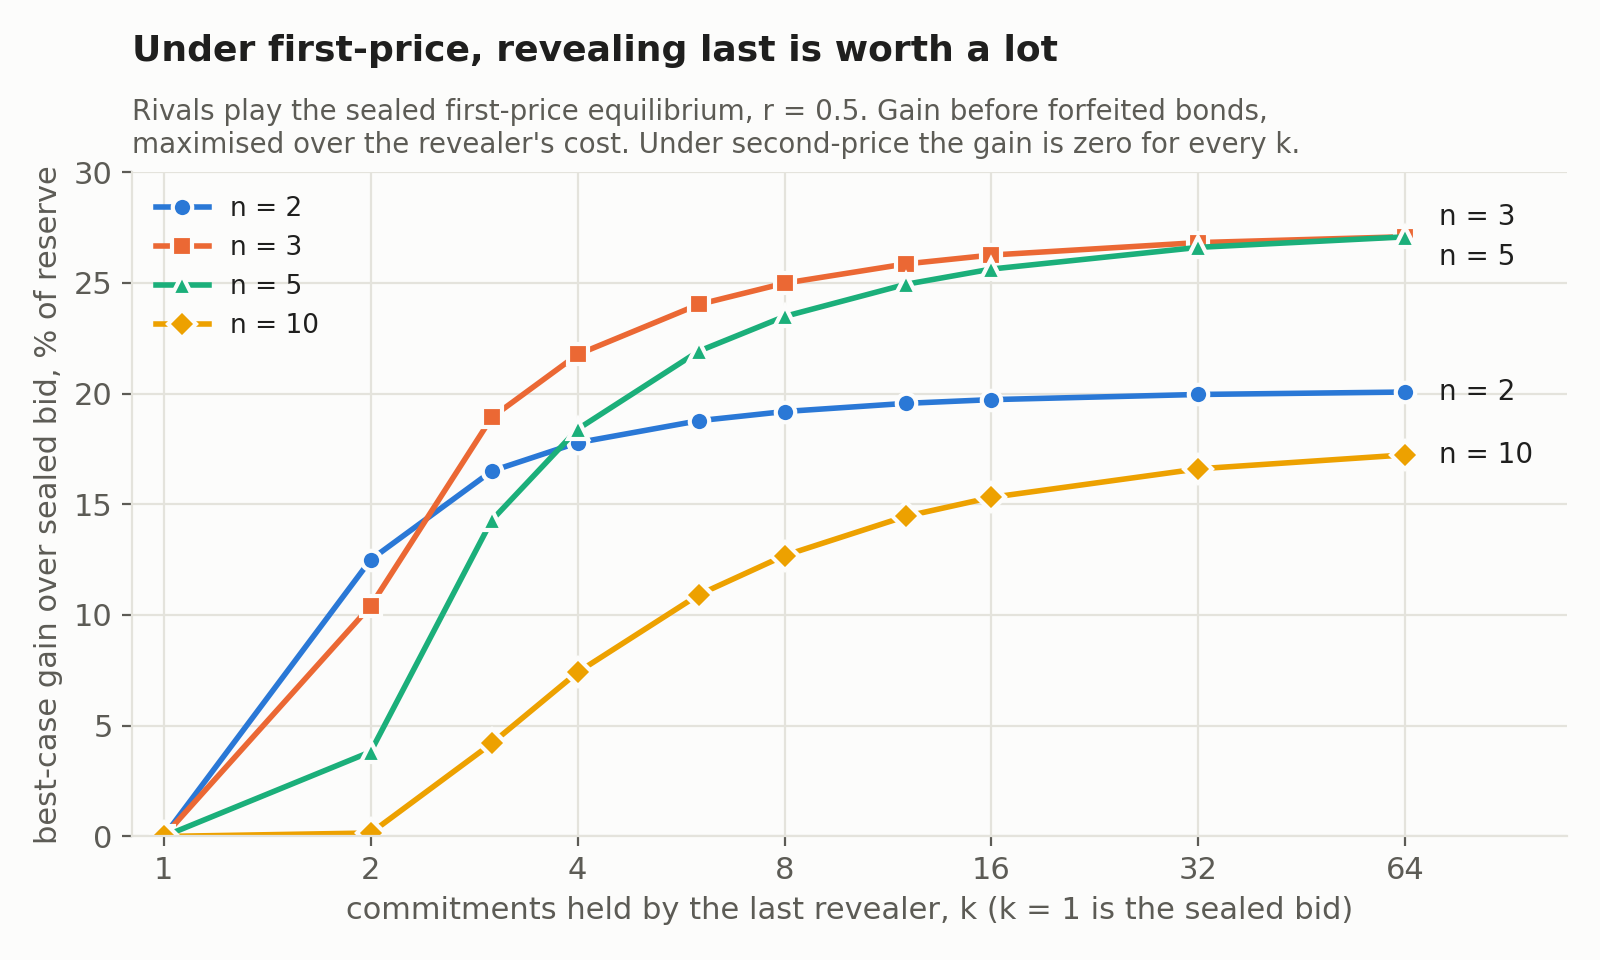
\includegraphics[width=0.8\linewidth]{fig-ladder.png}
\caption{Gain from holding $k$ commitments and revealing last, under first-price, as a share of the reserve. Under second-price the gain is zero for every $k$.}
\label{fig:ladder}
\end{figure}

\begin{table}[t]
\centering
\small
\begin{tabular}{@{}rcccc@{}}
\toprule
$n$ & $k = 4$ & $k = 16$ & $k = 64$ & bond to deter $k = 2$ \\
\midrule
2 & 17.8\% & 19.7\% & 20.1\% & 12.5\% \\
3 & 21.8\% & 26.3\% & 27.1\% & 10.4\% \\
5 & 18.4\% & 25.6\% & 27.1\% & 7.1\% \\
10 & 7.4\% & 15.3\% & 17.2\% & 2.5\% \\
\bottomrule
\end{tabular}
\caption{Interim gain of a last revealer with $k$ commitments under first-price, and the bond that makes a two-commitment ladder unprofitable, both as a share of the reserve.}
\label{tab:ladder}
\end{table}

\subsection{Dummy commitments}

A requester can post commitments it never intends to reveal, at the cost of the forfeited bonds. Under first-price, bidders who take the visible number of commitments at face value believe they face more competition and shade less. With three real bidders, three dummy commitments lower the requester's expected payment from 0.344 to 0.277, by 19\% (Figure~\ref{fig:phantom}). Under second-price the bids, and hence the payment, are unaffected. The same reasoning shows why forfeited bonds must not reach the requester, directly or indirectly: otherwise dummy commitments cost it nothing. The specification therefore makes the recipient of forfeited bonds a term every bidder sees, and forbids it to be any address from which the requester can recover funds.

\begin{figure}[t]
\centering
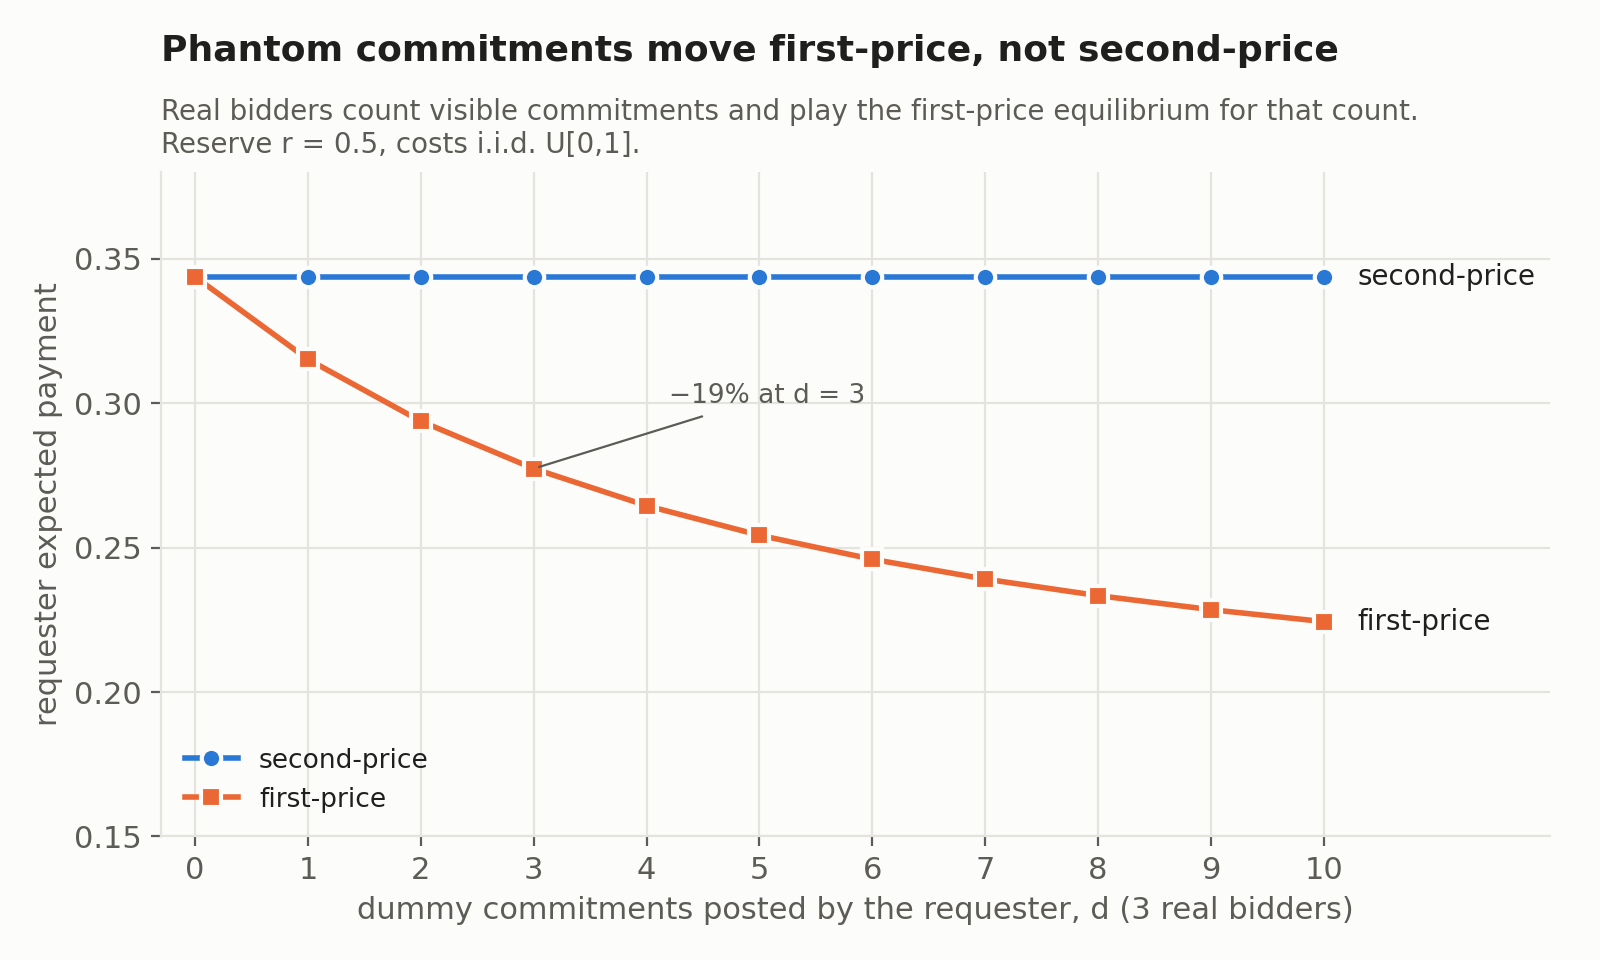
\includegraphics[width=0.75\linewidth]{fig-phantom.png}
\caption{Requester's expected payment against the number of dummy commitments, with three real bidders, under first-price and second-price.}
\label{fig:phantom}
\end{figure}

\subsection{False-name bids}
\label{sec:falsename}

The contract can tell addresses apart but not operators, so an operator can bid from several addresses \citep{yokoo2004}. Under uniform-price this breaks the unit-demand assumption behind truthfulness, and the operator can profit by withholding supply, which is demand reduction by another route \citep{ausubel2014}.

\begin{example}
Two units, reserve 100. An operator controls two addresses, committed before two rivals, and can perform each unit at cost 10. The rivals bid 10 and 30. If the operator bids 10 from both addresses, it wins both units at the clearing price 10 and earns nothing. If it bids 10 and 30, it wins one unit, its second address sets the clearing price at 30, and it earns 20. Sealing the bids does not help, because the operator can choose which commitment to open after seeing earlier reveals.
\end{example}

Single-unit second-price has no such weakness.

\begin{proposition}[False-name immunity]
\label{prop:falsename}
Under \code{award.vickrey} with one unit, an operator with cost $c$ that bids from any number of addresses earns no more than it earns bidding $c$ from a single address.
\end{proposition}

\begin{proof}
If none of the operator's addresses wins, it earns zero, which by Proposition~\ref{prop:vickrey} is at most its truthful single-address payoff. If address $i$ wins with bid $b_i$, the price is $\min(r, \min_{j \ne i} b_j)$, where the minimum runs over all other bids, including the operator's other addresses. Adding bids can only lower this minimum, so the operator earns at most $\min(r, m) - c$, where $m$ is the lowest rival bid; that is exactly what a single address bidding $b_i$ would earn, and by Proposition~\ref{prop:vickrey} no more than a single address bidding $c$.
\end{proof}

A brute-force search over a grid of costs, rival bids and two-address strategies in the reference implementation finds the uniform-price gain and confirms Proposition~\ref{prop:falsename} in 2,592 cases. Uniform-price with several units is therefore truthful only where an admission layer binds each operator to one address.

\section{Implementation and Verification}
\label{sec:impl}

The reference implementation \citep{repo} consists of the tender contract, the four mechanism contracts and two ERC-8414 adapters, in Solidity~0.8.24. The tender holds bidder bonds only and pays forfeited bonds through a separate permissionless claim, so that a recipient that rejects payment cannot block an award. It records the mechanism's code hash when the tender opens and refuses to finalize if the code has changed, and it re-checks every award against the revealed bids. A code hash does not reveal a proxy whose implementation can change behind it, so bidders must still inspect the mechanism's code; (C1) makes upgradeable mechanisms non-conforming. Finalization sorts the revealed bids, so its cost grows faster than linearly in the number of bidders: about 2 million gas at 128 revealed bids, 8 million at 256, 31 million at 512 and 122 million at 1,024. Each tender therefore sets a cap on bidders, limited to 256 in the reference implementation.

Table~\ref{tab:lean} lists the machine-checked results. The proofs use core Lean~4 (v4.34.0) without Mathlib, contain no unproved steps, and depend only on Lean's standard axioms. The model of \code{award.vickrey} in Lean takes one bidder's view, splitting the other bids into those committed before and after it, which is how the tie rule enters; the correspondence between this model and the Solidity contract is checked on a finite grid by the test suite. The test suite comprises 1,037 assertions run against the contracts in an in-process EVM---golden vectors for all four rules, the seven conditions over an exhaustive three-bidder grid, brute-force dominance checks, the full tender lifecycle and both adapters---and 30 Foundry tests, including fuzzed monotonicity and truthfulness, faulty mechanisms and a mechanism whose code is replaced after opening.

\begin{table}[t]
\centering
\small
\begin{tabular}{@{}ll@{}}
\toprule
Theorem & Statement \\
\midrule
\code{truthful\_dominant} & Truthful bidding is weakly dominant under \code{award.vickrey} \\
\code{truthful\_nonneg} & Truthful bidding never yields a negative payoff \\
\code{wins\_of\_le} & Lowering a winning bid keeps it winning (C5) \\
\code{price\_le\_reserve} & The price never exceeds the reserve (C3) \\
\code{bid\_le\_price\_of\_wins} & A winner is never paid less than its bid (C7) \\
\code{fixed\_reward\_not\_truthful} & Bid ranking with a fixed reward is not truthful \\
\code{fixed\_reward\_lowest\_bid\_weakly\_better} & With a fixed reward, the lowest bid weakly dominates \\
\code{posted\_price\_acceptance\_dominant} & Accepting iff $c \le r$ is weakly dominant under posted price \\
\bottomrule
\end{tabular}
\caption{Results machine-checked in Lean 4.}
\label{tab:lean}
\end{table}

\section{Discussion and Limitations}

The analysis assumes independent private costs and risk-neutral bidders. Agents built on the same model API may have strongly correlated costs, which weakens the case for second-price and makes bidding rings easier to sustain; requesters should set the reserve from their own outside option rather than from observed past prices. The numerical results use uniform costs and a simple deviation model, and the ladder figures are lower bounds on what a well-placed ladder gains. The commit--reveal procedure leaves bids public at reveal time; encrypted reveals, for example with threshold or fully homomorphic encryption, would make first-price usable but are outside the interface. The content hash relies on the consuming standard to commit to task content, which ERC-8414 does not yet do, and false-name resistance for multi-unit rules needs an identity layer that this interface deliberately leaves out.

More broadly, the composition conditions are not specific to these standards. Whenever an auction is computed by one module and executed by another, the executing module inherits the burden of commitment: it must pay what the mechanism says, execute what it decides, and leave the object unchanged once bids are in. Stating these as declared profiles, checked when a tender opens, makes the burden visible to bidders before they commit.

\section{Conclusion}

We have proposed a sealed-bid award interface for on-chain agent task markets and shown that its incentive properties hold only under conditions on the market that consumes the award. A consumer that pays a fixed reward can use only a posted price; a consumer that pays the award price must also be committed to executing every award on content fixed at opening. On a public ledger, single-unit second-price is robust to sequential reveals, dummy commitments and multiple addresses, while first-price and uniform-price are not. The interface, its integration profiles and the reference implementation are under public review as a draft Ethereum standard.

\section*{Acknowledgements}

The composition conditions and several robustness results arose from public review of the draft standard on the Ethereum Magicians forum. The author thanks SergeevDmitry for the fixed-reward counterexample; chugarchugarr for the split into price-binding and allocation-only integrations and for the terms payment-binding and execution-binding; predge-ai for the question of award finality; Revinand for identifying missing award checks and the assumption of mechanism immutability; zexoverz for the false-name argument against uniform-price; Ted (ted0x) for the case of a task changed after the award; and Garyyang for discussion of ERC-8414. Any errors are the author's. The author used an AI assistant for drafting text and code; all content was reviewed by the author.

\paragraph{Code and data availability.} The draft standard, reference implementation, proofs, tests and analysis scripts are available at \url{https://github.com/shentonyan/sealed-bid-award-erc} under CC0.

\bibliographystyle{plainnat}
\bibliography{refs}

\end{document}
\typeout{get arXiv to do 4 passes: Label(s) may have changed. Rerun}
